\section{结果}

\begin{figure*}[!t]
\centering
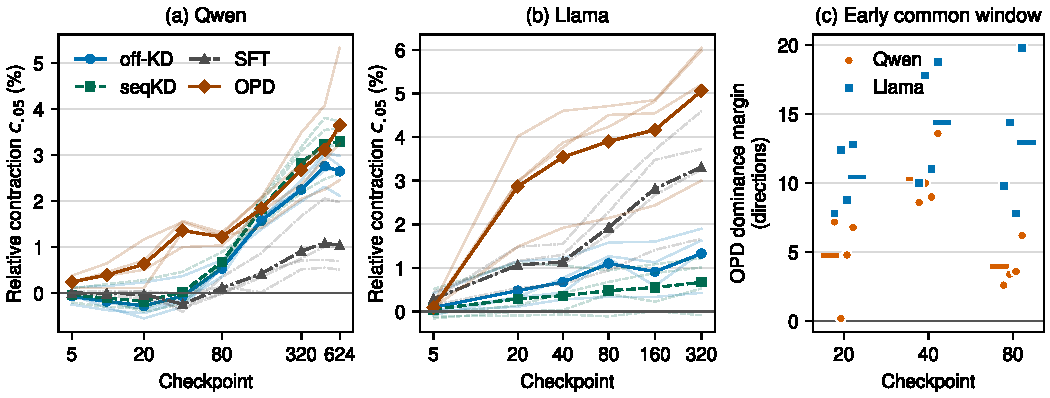
\includegraphics[width=\textwidth]{figures/fig1_main_trajectories.pdf}
\caption{纯激活、纯权重与功能轨迹。上行为 Qwen，下行为 Llama；各列依次为 activation ER、TPNT 相对 null 的 excess lift、PABS drift $10^4(1-\mathrm{PABS})$ 和 equal-5 相对功能压缩。四列量纲不同，原始纵轴幅度不可跨列比较；曲线仅连接实际 checkpoint。功能谱呈现了前三类坐标未共同复现的训练设置分离。}
\label{fig:main}
\end{figure*}

\begin{table*}[!t]
\centering
\small
\setlength{\tabcolsep}{5pt}
\begin{tabular}{lccc}
\toprule
模型 & Activation suite $A$ & Functional $C_5$ & Weight $P_{k,5}$ \\
\midrule
Llama & .556 & \textbf{.743} & .688 \\
Qwen & .595 & \textbf{.708} & .521 \\
\bottomrule
\end{tabular}
\caption{严格共同网格上的 OPD 识别（checkpoint-held-out AUC）。每个模型使用 64 个共同状态、相同 equal-5 模块和 folds。$A$ 是包含 ER、PR、top-1/8/32 share、raw/centered anisotropy 与 step-0 CKA 的八维纯激活特征组，不是图~\ref{fig:main} 中的 ER 单项。}
\label{tab:identification}
\end{table*}

\begin{table*}[!t]
\centering
\small
\setlength{\tabcolsep}{4pt}
\begin{tabular}{lrrrrr}
\toprule
模型 & $M_{\min}^{\mathrm{early}}$ & OPD NCD & SFT NCD & off-KD NCD & seqKD NCD \\
\midrule
Qwen & .200 & \textbf{50.423} & 9.554 & 31.017 & 37.793 \\
Llama & 7.800 & \textbf{77.594} & 39.683 & 17.518 & 11.093 \\
\bottomrule
\end{tabular}
\caption{共同早期排序与全轨迹压缩剂量。$M_{\min}^{\mathrm{early}}$ 是四核心域和共同早期 checkpoint 上的最小 OPD 连续边际（directions）；正值排除该范围内的排序反转。NCD 在 $\log(1+t)$ 上积分至 $T=320$（directions$\times$log-step），衡量压缩深度与持续时间。两列尺度不可直接比较。}
\label{tab:ncd}
\end{table*}

\begin{figure*}[!t]
\centering
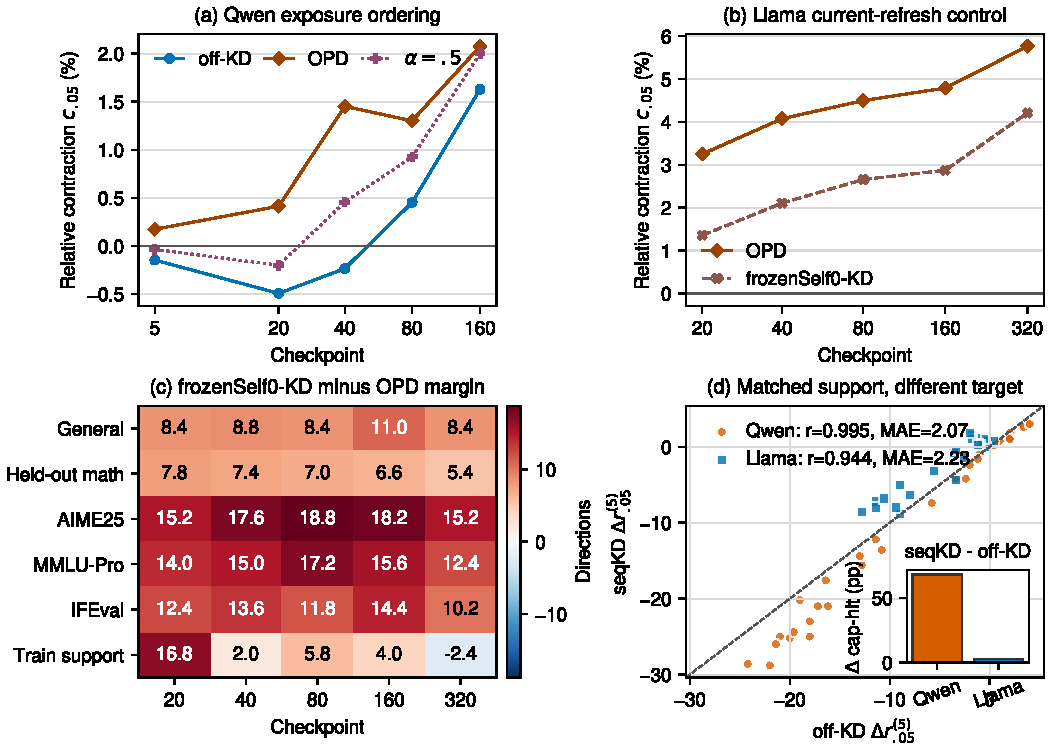
\includegraphics[width=\textwidth]{figures/fig2_support_controls.pdf}
\caption{Sequence exposure 与 refresh 对照。（a）Qwen $\alpha=.5$ 相对 off-KD 和 OPD 的有序轨迹。（b）Llama OPD 与 frozenSelf0-KD 在五个固定外部域上的等域平均绝对轨迹。（c）对应的逐域配对边际；正值表示持续刷新的 OPD 更压缩，粗黑线为外部域均值。图例中的 Math、AIME、MMLU 和 Mean 分别表示 held-out math、AIME25、MMLU-Pro 和五域均值。}
\label{fig:controls}
\end{figure*}

\begin{table*}[!t]
\centering
\small
\setlength{\tabcolsep}{2.7pt}
\textbf{A. off-KD 与 seqKD 的逐域 equal-5 路径一致性（Pearson $r$/MAE directions）}\\[2pt]
\begin{tabular}{lccccc}
\toprule
模型 & General & Math & MMLU-Pro & IFEval & Pooled \\
\midrule
Qwen & .995/1.13 & .996/2.67 & .998/2.18 & .999/2.29 & .995/2.07 \\
Llama & -.771/2.53 & .971/1.73 & .968/2.23 & .824/2.40 & .944/2.23 \\
\bottomrule
\end{tabular}

\vspace{4pt}
\textbf{B. 匹配训练设置的终点行为（\%）}\\[2pt]
\begin{tabular}{llrrrrrrr}
\toprule
模型 & 设置 & \multicolumn{2}{c}{MATH500} & \multicolumn{3}{c}{MMLU-Pro} & \multicolumn{2}{c}{IFEval} \\
\cmidrule(lr){3-4}\cmidrule(lr){5-7}\cmidrule(lr){8-9}
 & & Acc. & Cap & Strict & Flex. & Extract & Prompt & Instr. \\
\midrule
Qwen & off-KD & 79.4 & 4.8 & 35.4 & 57.1 & 47.3 & 23.1 & 36.5 \\
 & seqKD & 72.4 & 73.0 & 30.6 & 58.1 & 54.1 & 24.4 & 39.3 \\
Llama & off-KD & 8.2 & 91.8 & 14.2 & 16.4 & 50.3 & 19.6 & 33.2 \\
 & seqKD & 10.2 & 94.6 & 13.1 & 15.4 & 51.6 & 19.2 & 31.5 \\
\bottomrule
\end{tabular}
\caption{Matched-support 的功能路径与行为读出。A 使用完全匹配的非零 checkpoint；MAE 是逐 checkpoint 的方向差。B 使用 Qwen step 624 与 Llama step 320；Cap 为 generation-cap hit，Extract 为 extraction failure，Prompt/Instr. 为 IFEval prompt/instruction strict。}
\label{tab:support-readout}
\end{table*}

\begin{figure*}[!t]
\centering
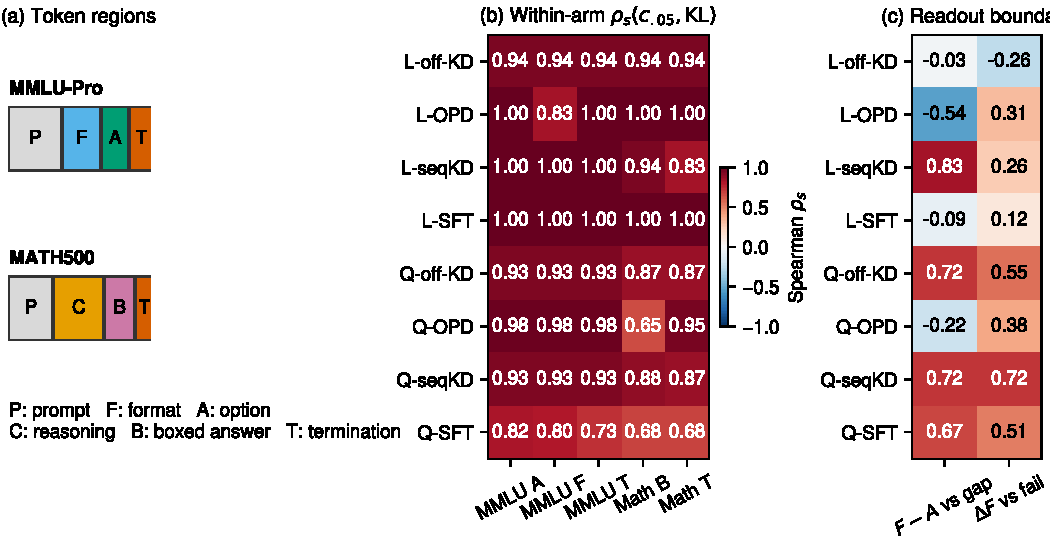
\includegraphics[width=\textwidth]{figures/fig3_regional_output.pdf}
\caption{区域输出关系。（a）每个模型和训练设置内，equal-5 功能压缩与区域 full-vocabulary KL 的跨 checkpoint Spearman。MMLU-Pro 的列为格式 $F$、正确选项标签 $A$ 和终止 $T$；MATH500 的列为推理 $C$、boxed answer $B$ 和终止 $T$。（b）MMLU-Pro 格式--答案 signed-NLL contrast 与 strict--flexible gap，以及格式 NLL 与 extraction failure 的相关。L 和 Q 分别表示 Llama 与 Qwen；每格数值给出相关系数。}
\label{fig:regional}
\end{figure*}

\begin{table*}[!t]
\centering
\small
\setlength{\tabcolsep}{4pt}
\begin{tabular}{llcc}
\toprule
模型/域 & 区域 & Held-out $R^2$: $C_5$ & Best $P_{k,5}$ \\
\midrule
Llama / MMLU-Pro & $A/F/T$ & \textbf{.869/.932/.468} & .743/.788/.459 \\
Llama / MATH500 & $B/T$ & .561/\textbf{.812} & \textbf{.615}/.647 \\
Qwen / MMLU-Pro & $A/F/T$ & \textbf{.426/.577/.596} & .243/.318/.443 \\
Qwen / MATH500 & $B/T$ & \textbf{.227}/.604 & .167/\textbf{.718} \\
\bottomrule
\end{tabular}
\caption{区域 full-vocabulary KL 的样本外预测。$C_5$ 与 $P_{k,5}$ 使用相同五模块、共同状态和 checkpoint-held-out folds。数值按区域顺序排列；粗体为逐区域更高的 $R^2$。后补 Math $C$ 的轨迹内和 checkpoint-demeaned 结果在正文报告，其 matched held-out 横向比较不在本表中。}
\label{tab:regional-prediction}
\end{table*}


\subsection{功能谱提供纯激活与纯权重坐标之外的轨迹信息}

图~\ref{fig:main} 将相同训练设置和 checkpoint 上的四种观察量并列。ER 记录激活协方差的谱维数；TPNT 记录更新坐标在 source principal mask 上的富集；PABS 记录主权重子空间的旋转；功能谱则记录当前权重在域上实际访问方向中形成的输出模式。前三者不能通过纵轴幅度与功能谱直接比较，但可以比较它们是否产生一致的训练轨迹结构。

纯激活轨迹没有复现功能谱的分离。Llama 多个外部域中，OPD@160 的 ER 相对变化不足 $.003$，step-0 CKA 仍约为 $.9997$--$1.0000$，而相同位置的 $r_{.05}$ 已减少约 14--26 个方向。TPNT 在部分 checkpoint 出现高于 spectrum-matched null 的局部富集，但未形成跨模型稳定的 OPD 特异轨迹；PABS 始终接近 1，配套 NSS 也很小，说明当前 LoRA 轨迹主要在近乎固定的主权重基底内演化。相较之下，图~\ref{fig:main} 最后一列中的 equal-5 功能压缩呈现清楚的训练设置分离。该差异来自 $W_t$ 与域输入度量的共同作用，而非更多同类特征。完整原生指标、null 与层级结果见 Supplementary Secs.~B.4 与 C.3。

在两个模型各 64 个严格共同状态上，我们进一步按 checkpoint group 留出训练阶段。完整 activation suite $A$、功能压缩 $C_5$ 与 source-principal block $P_{k,5}$ 的 OPD 识别结果见表~\ref{tab:identification}。$C_5$ 在两模型中都提供更清楚的排序判别；在三个输出目标的同协议比较中，它也均优于 raw activation block。strict $p_k$ 仍保留 Qwen absolute-NLL 的局部优势，说明功能状态与权重位置提供任务依赖的互补信息，而非普遍支配关系（Supplementary Sec.~D.3）。

\subsection{OPD 支配共同早期功能压缩}

图~\ref{fig:main} 最后一列显示，两种模型中的 OPD 都在共同早期窗口进入更深的功能压缩状态。为检验域平均是否掩盖排序反转，定义 OPD 相对最接近离线设置的边际
\begin{equation}
M_{m,D,t}
=\min_{b\in\{\mathrm{SFT,offKD,seqKD}\}}\Delta r_{m,b,D,t}^{(5)}
-\Delta r_{m,\mathrm{OPD},D,t}^{(5)}.
\end{equation}
$M>0$ 表示 OPD 比每个离线设置都更压缩。在 $\varepsilon=.05$ 下，两模型四域和 step 20/40/80 的最小边际均为正；完整逐域曲线见 Supplementary Sec.~C.1。为概括完整轨迹，我们再在 $\tau=\log(1+t)$ 上积分基线以下压缩至 $T=320$，得到 negative contraction dose（NCD）。表~\ref{tab:ncd} 分别保留早期排序和全程剂量：OPD 在两模型中都具有最大 NCD。

四个阈值、连续谱、centered covariance 与层级审计保持这一结论；逐模块结果表明 OPD 最深的排序在 value/output 与 MLP 中更稳定，而 q/k 具有异质性。它不表示压缩能量只来自五类模块。完整 equal-7、层级和模块结果见 Supplementary Secs.~C.2--C.3。

\subsection{Exposure 与 Refresh 组织轨迹，但不决定读出}

在相同 forward-KL 下，Qwen 的 $\alpha=.5$ 轨迹沿 off-KD 到 OPD 有序移动，但并非严格一维插值（图~\ref{fig:controls}a）。Llama frozenSelf0-KD 则只移除 current-student rollout 的持续刷新。OPD 相对 frozenSelf0-KD 的压缩优势在五个固定外部域和全部后续 checkpoint 上持续存在（图~\ref{fig:controls}b--c），因此 current-support refresh bundle 是更直接的组织因素。由于 refresh 同时改变 rollout 长度、EOS、重复与风格，该对照识别的是总体 refresh bundle，而不是纯粹的 freshness 效应。

off-KD 与 seqKD 使用完全相同的 teacher sequences、顺序、步数和 LoRA 配置，只改变监督目标。表~\ref{tab:support-readout}A 显示，二者在 Qwen 四个核心域中形成高度一致的功能路径；Llama 的模式预算总体接近，但 General 域的时间同动具有异质性。行为读出并未被这些路径锁定：Qwen 的 seqKD 在终点出现显著更高的 MATH500 cap-hit，并伴随 accuracy 和格式读出的变化，而 Llama 没有复现同等幅度的分叉（表~\ref{tab:support-readout}B）。相同 sequence support 可以组织相近的功能模式预算，target distribution 仍能改变具体读出。

\subsection{相对功能压缩追踪区域无符号输出移动}

图~\ref{fig:regional}a 比较 $c_{.05}^{(5)}$ 与区域 KL 在每条训练设置内的相关。MMLU 的格式、答案和终止，以及 MATH 的推理、boxed answer 和终止，大多数都随功能压缩同步移动；Math CoT 区域在两个模型的四种设置中也全部为正。为固定训练阶段，我们在每个 model--domain--checkpoint 内减去同期四设置均值。Math $\mathrm{KL}_C$ 的相关在 Llama/Qwen 中仍为 $.875/.573$，而 $\mathrm{KL}_B$ 为 $.902/.440$；regional contrast $\mathrm{KL}_B-\mathrm{KL}_C$ 则为 $-.209/-.183$。因此功能压缩追踪各区域移动了多少，却不决定移动主要分配到推理还是最终答案。

表~\ref{tab:regional-prediction}进一步在原先冻结的实际 KL 区域上比较 $C_5$ 与强权重基线 $P_{k,5}$。功能谱在大多数区域取得更高样本外 $R^2$，明确例外是 Llama Math boxed-answer 与 Qwen Math termination。该横向比较尚不包含后补的 Math $C$，因而不把新区域并入旧胜负汇总。扩展到 signed 与 absolute targets 后，两个坐标的平均差距缩小；完整固定参考序列合并为单一区域时，无符号关系仍然存在（Supplementary Secs.~D.1--D.3）。

\subsection{Signed Readout 与真实行为具有模型依赖性}

KL 测量移动幅度；signed NLL 进一步询问 reference token 变得更容易还是更困难。MMLU-Pro 的 $\Delta\mathrm{NLL}_{F-A}$ 对比格式与答案区域，MATH 的 $\Delta\mathrm{NLL}_{B-C}$ 对比 boxed answer 与之前推理。它们到 strict--flexible gap 或 extraction failure 的关系在模型和训练设置之间改变符号（图~\ref{fig:regional}b）。例如，$F-A$ 在 Qwen off-KD/seqKD 中与格式缺口正相关，却在 Qwen OPD 和 Llama OPD 中负相关。功能模式数量、区域分配、reference-token 读出效价和自由生成行为因而是相关但不可合并的层次。

这一边界与 matched-support 结果一致。功能谱可以描述 sequence support 如何组织局部模式预算，以及输出分布移动了多少，但单一 rank 不能判断这些移动改善还是损伤任务。Qwen adapter zeroing 和答案位概率质量审计进一步支持格式/readout 通道解释，但属于模型特定的补充证据（Supplementary Sec.~D.5）。
